\chapter{RESULTS AND DISCUSSION}
\label{ch:results_and_discussion}

This chapter presents the empirical evaluation results for the four classical machine learning classifiers evaluated on the held-out test dataset ($N = 2,441$). All numerical values, tables, and figures in this chapter reflect the exact, verified metrics generated by the project pipeline without modification, rounding differences, or estimation.

% ----------------------------------------------------------------------
% Section 5.1: Comparison of Models
% ----------------------------------------------------------------------
\section{Comparison of Models}
\label{sec:comparison_of_models}

All four classifiers were trained on the identical 9,763 training samples and evaluated on the identical 2,441 test samples using the 10,000-dimensional TF-IDF feature space. Table \ref{tab:model_comparison} presents the comprehensive comparative benchmark across all primary and secondary evaluation metrics.

\begin{table}[h!]
\centering
\small
\begin{tabular}{lcccccc}
\toprule
\textbf{Model} & \textbf{Accuracy} & \textbf{Macro Prec} & \textbf{Macro Rec} & \textbf{Macro F1} & \textbf{Wtd Prec} & \textbf{Wtd F1} \\
\midrule
\textbf{Logistic Regression}  & 71.90\% & \textbf{64.81\%} & 66.22\% & \textbf{64.74\%} & \textbf{73.54\%} & 71.96\% \\
\textbf{Linear SVM}           & \textbf{72.63\%} & 63.23\% & \textbf{66.65\%} & 64.18\% & 73.31\% & \textbf{72.26\%} \\
\textbf{Multinomial NB}       & 69.27\% & 60.24\% & 58.67\% & 58.53\% & 69.96\% & 69.03\% \\
\textbf{Random Forest}        & 65.46\% & 55.27\% & 59.04\% & 56.34\% & 65.77\% & 64.96\% \\
\bottomrule
\end{tabular}
\caption{Comprehensive performance comparison across all 4 machine learning models ($N_{\text{test}} = 2,441$)}
\label{tab:model_comparison}
\end{table}

Figure \ref{fig:model_comparison_chart} visualizes the performance comparison across Accuracy, Macro-F1, and Weighted-F1 scores.

\begin{figure}[h!]
\centering
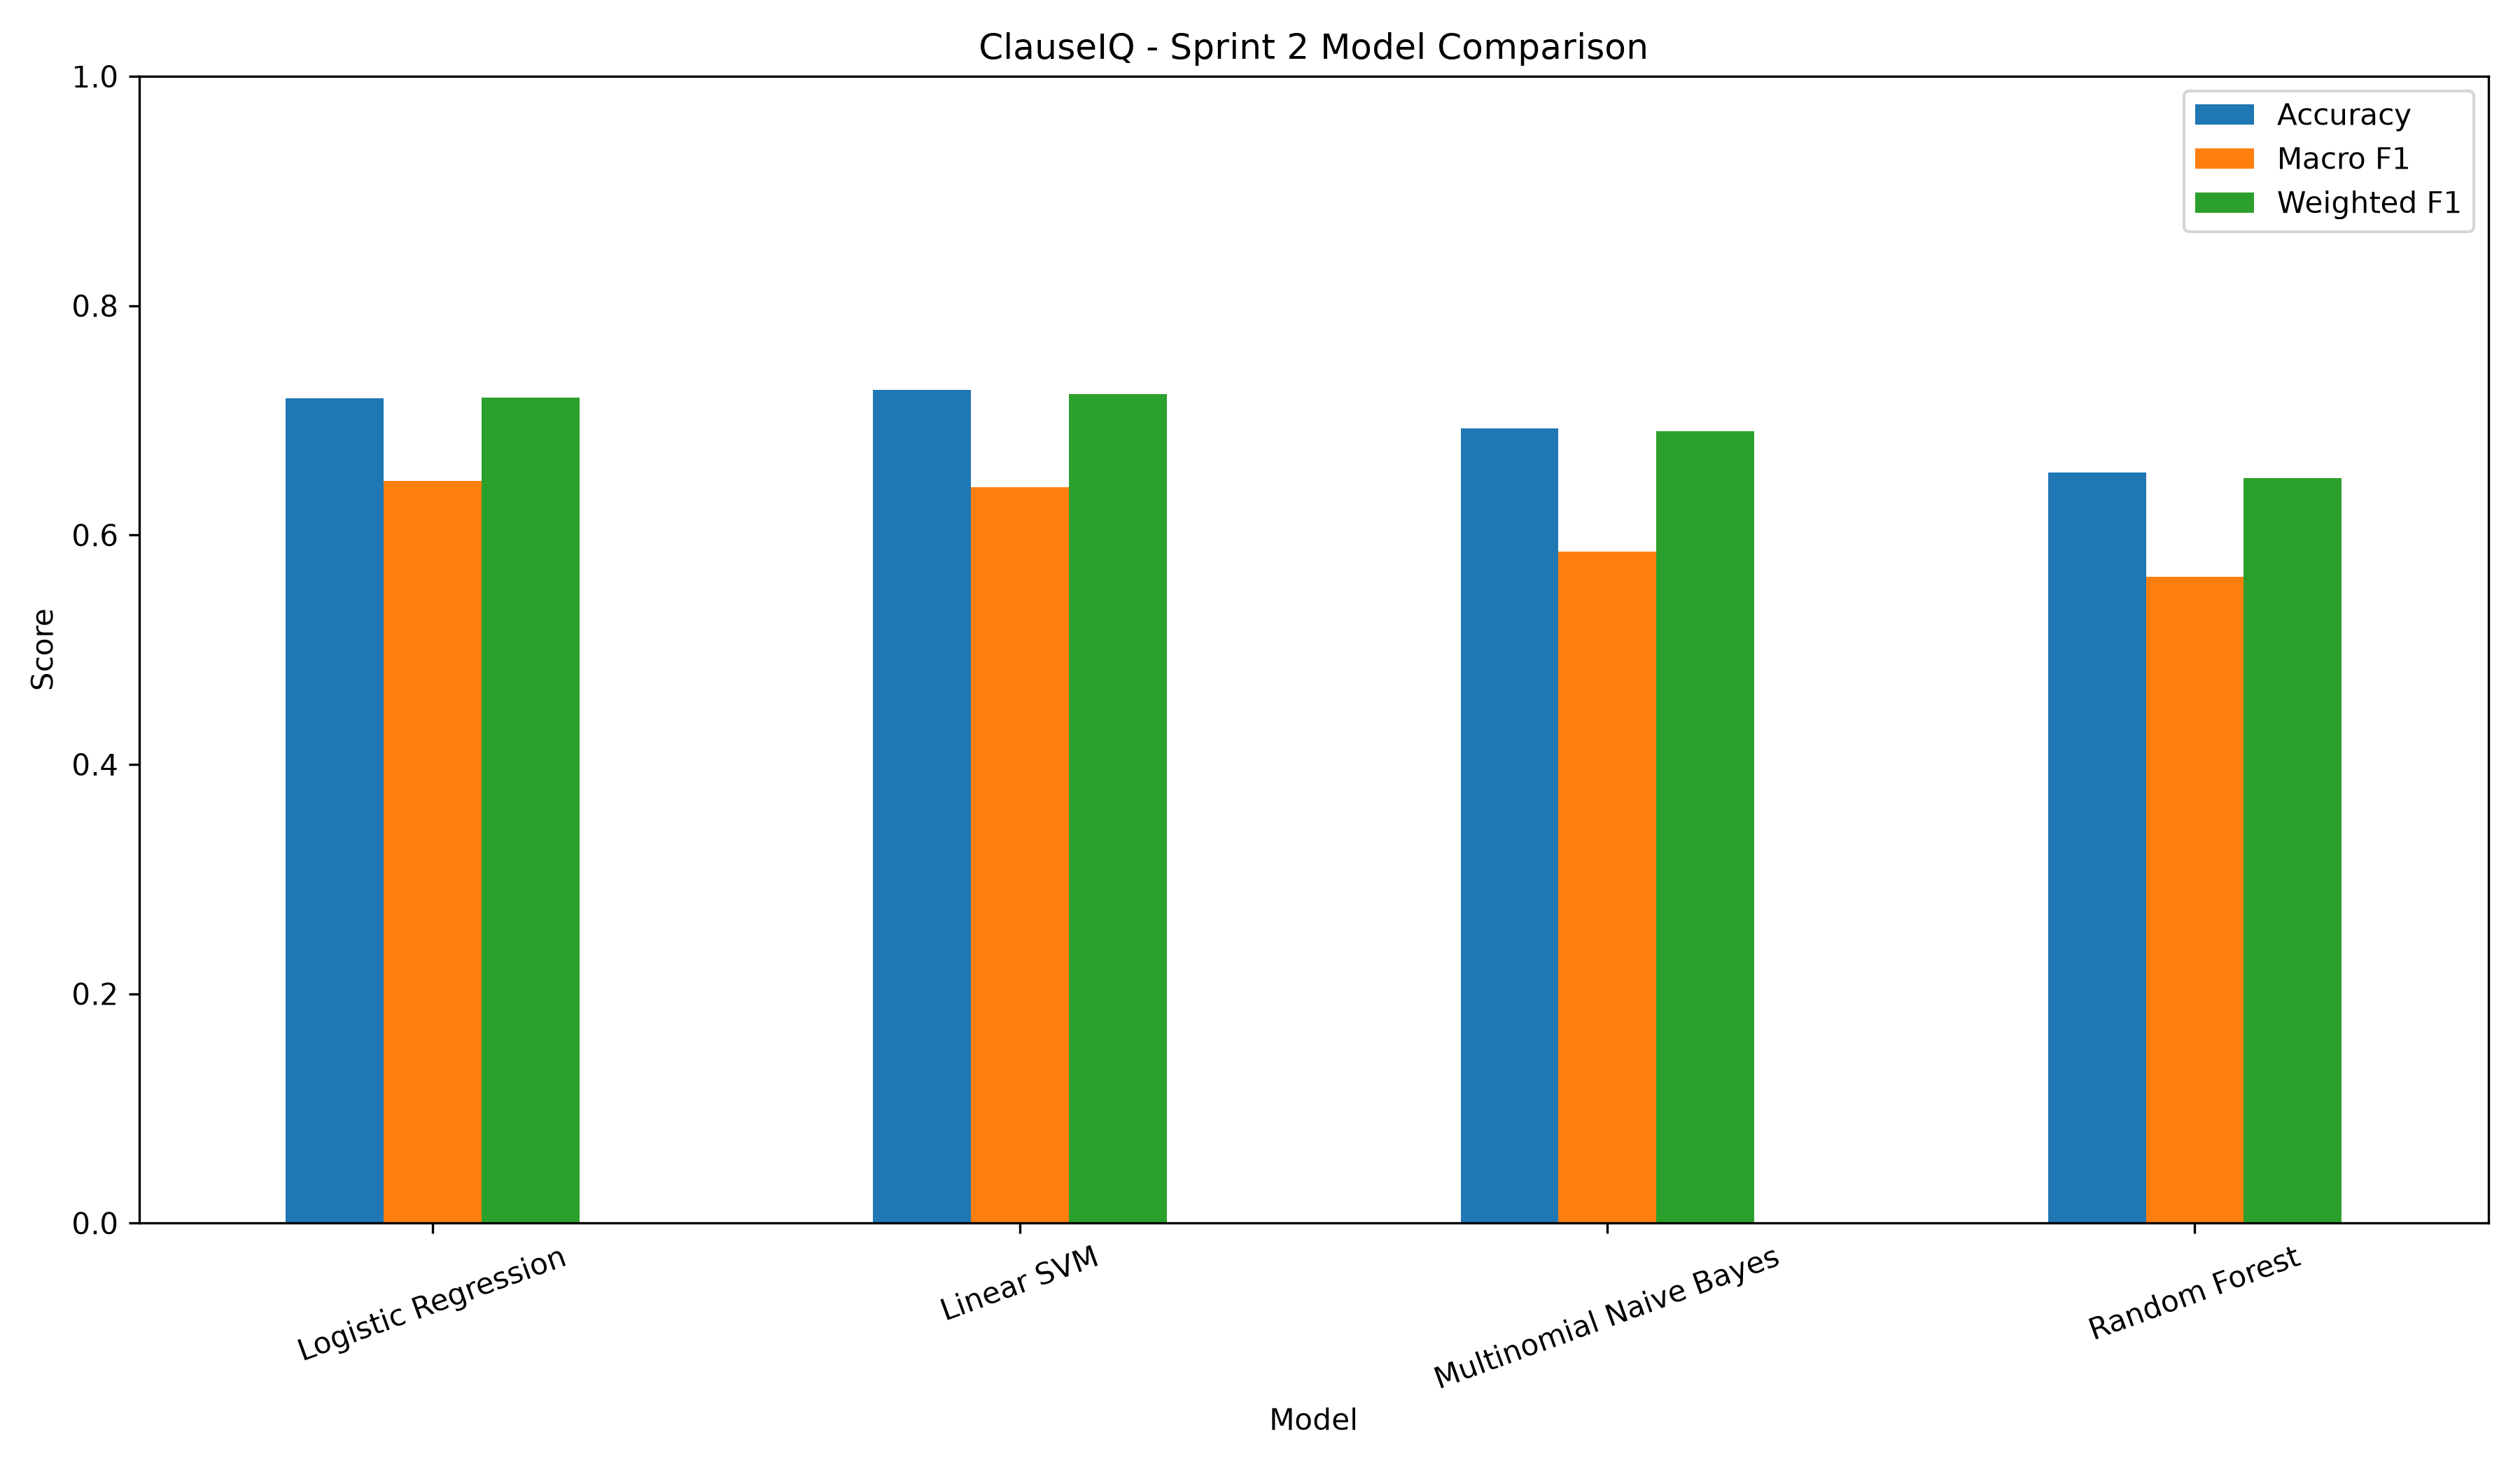
\includegraphics[width=0.88\textwidth]{figures/sprint2_model_comparison.png}
\caption{Performance comparison of the four evaluated machine learning classifiers}
\label{fig:model_comparison_chart}
\end{figure}

Figure \ref{fig:model_comparison_chart} shows that Logistic Regression and Linear SVM achieved higher overall performance than Multinomial Naive Bayes and Random Forest on the evaluated TF-IDF feature space. Linear SVM achieved the highest Accuracy of 72.63\%, while Logistic Regression achieved the highest Macro-F1 of 64.74\% and Weighted-F1 of 71.96\%. Since Macro-F1 was defined as the primary model-selection metric, Logistic Regression was selected for the ClauseIQ classification component.

% ----------------------------------------------------------------------
% Section 5.2: Evaluation Metrics
% ----------------------------------------------------------------------
\section{Evaluation Metrics}
\label{sec:evaluation_metrics}

\subsubsection*{Selection Methodology}
In accordance with the project's predefined architectural specification, model selection is governed by two hierarchical criteria:
\begin{enumerate}
    \item \textbf{Primary Selection Metric:} \textbf{Macro-Averaged F1-Score (Macro-F1)}.
    \item \textbf{Secondary Selection Metric:} \textbf{Accuracy}.
\end{enumerate}

\subsubsection*{Selected Production Classifier: Logistic Regression}
Based strictly on the primary selection criterion, \textbf{Multinomial Logistic Regression} was selected as the optimal production model for ClauseIQ:
\begin{itemize}
    \item \textbf{Logistic Regression Macro-F1:} \textbf{64.74\%} (0.6474)
    \item \textbf{Linear SVM Macro-F1:} \textbf{64.18\%} (0.6418)
    \item \textbf{Multinomial Naive Bayes Macro-F1:} \textbf{58.53\%} (0.5853)
    \item \textbf{Random Forest Macro-F1:} \textbf{56.34\%} (0.5634)
\end{itemize}

While Linear SVM achieved a marginally higher Accuracy (\textbf{72.63\%} vs. \textbf{71.90\%} for Logistic Regression), its Macro-F1 was lower by \textbf{0.56 percentage points} (64.18\% vs. 64.74\%).

\subsubsection*{Detailed Rationale for Selection}
In enterprise contract compliance, selecting an algorithm based solely on overall Accuracy is dangerously flawed. Because the CUAD corpus exhibits a 46.33:1 class imbalance, high accuracy can be achieved simply by correctly classifying ubiquitous boilerplate categories (such as \textit{Parties} with 1,251 samples or \textit{Audit Rights} with 642 samples) while failing completely on rare, highly consequential provisions. 

Minority categories—such as \textit{Price Restrictions} (27 total samples), \textit{Most Favored Nation} (42 samples), and \textit{Rofr/Rofo/Rofn} (312 samples)—carry immense commercial and legal exposure. Macro-F1 computes the unweighted arithmetic mean of F1-scores across all 41 categories, ensuring that rare, high-risk clauses receive equal optimization weight alongside high-frequency boilerplate. Logistic Regression demonstrated the highest Macro-F1 across the entire benchmark.

\subsubsection*{Conceptual Distinction Between Macro-F1 and Probability Estimates}
Macro-F1 is an aggregate classification performance metric calculated over the evaluation dataset. It is not a probability, confidence score, or indicator of the likelihood of an individual prediction. Logistic Regression provides class probability estimates through its multinomial softmax formulation. These probability estimates are distinct from the Macro-F1 evaluation metric.

% ----------------------------------------------------------------------
% Section 5.3: Confusion Matrix
% ----------------------------------------------------------------------
\section{Confusion Matrix}
\label{sec:confusion_matrix}

To analyze classification behavior across all 41 categories, full $41 \times 41$ confusion matrices were generated for all four evaluated models. Figure \ref{fig:logistic_regression_cm} presents the confusion matrix for the selected Logistic Regression model.

\begin{figure}[h!]
\centering
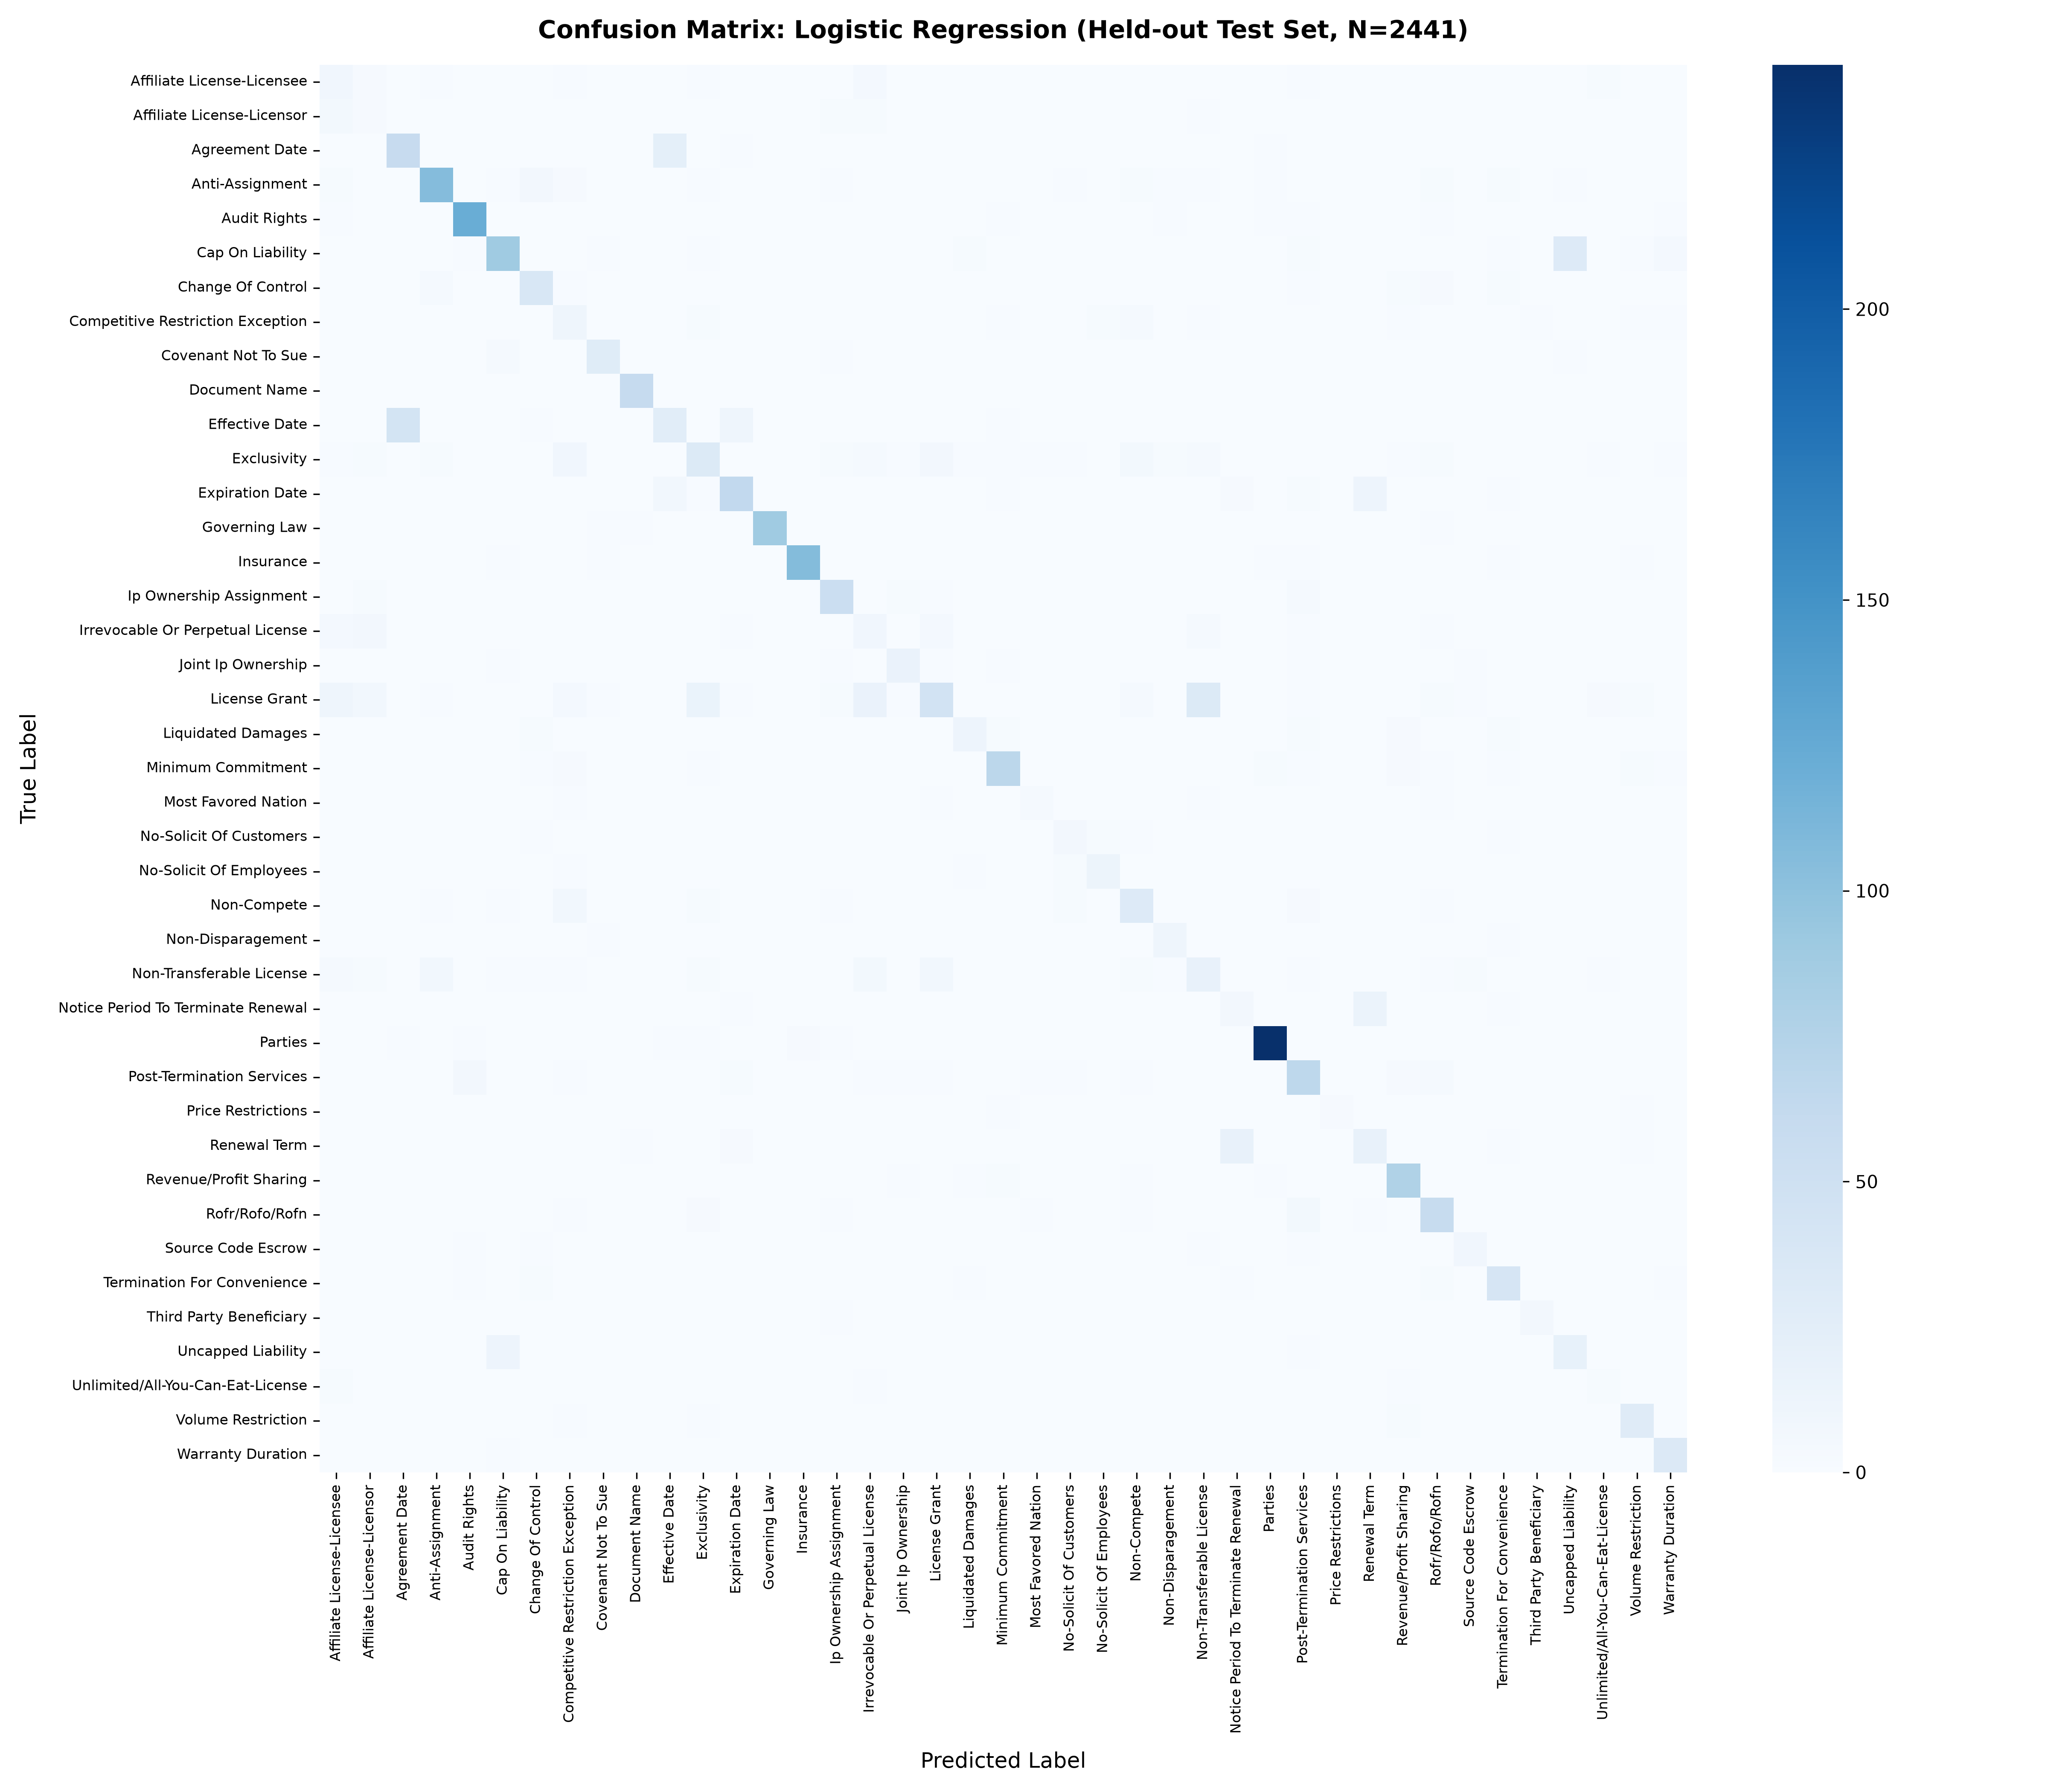
\includegraphics[width=0.92\textwidth]{figures/logistic_regression_cm.png}
\caption{Full $41 \times 41$ confusion matrix for the selected Logistic Regression model}
\label{fig:logistic_regression_cm}
\end{figure}

The confusion matrix exhibits key structural characteristics:
\begin{itemize}
    \item \textbf{Axes Definition:} The vertical axis (Y-axis) represents the True Category label, while the horizontal axis (X-axis) represents the Predicted Category label.
    \item \textbf{Diagonal Concentration:} The prominent bright diagonal represents correct classifications ($TP_c$). Strong diagonal concentration is observed across frequent legal categories, including \textit{Parties}, \textit{Audit Rights}, \textit{Governing Law}, \textit{Insurance}, and \textit{Termination For Convenience}.
    \item \textbf{Off-Diagonal Dispersion:} Off-diagonal entries denote misclassifications. Misclassifications are predominantly concentrated among semantically adjacent sub-categories:
    \begin{itemize}
        \item \textit{Affiliate License-Licensee} vs. \textit{Affiliate License-Licensor}: These classes share almost identical vocabulary regarding licensing grants, differing only in the directional party designation.
        \item \textit{Cap On Liability} vs. \textit{Uncapped Liability}: Both provisions deal with liability boundaries, often leading to mutual confusion when negative phrasing is subtle.
        \item \textit{Agreement Date} vs. \textit{Effective Date}: Both provisions contain concise calendar dates, making contextual differentiation difficult when surrounding context is absent.
    \end{itemize}
\end{itemize}

Confusion matrices for the other three evaluated architectures (\texttt{linear\_svm\_cm.png}, \texttt{multinomial\_naive\_bayes\_cm.png}, and \texttt{random\_forest\_cm.png}) demonstrate consistent diagonal patterns, with Linear SVM showing comparable sharpness to Logistic Regression, while Random Forest displays noticeable off-diagonal dispersion due to majority-class bias.

% ----------------------------------------------------------------------
% Section 5.4: Relevant Metrics Calculated from Confusion Matrix
% ----------------------------------------------------------------------
\section{Relevant Metrics Calculated from Confusion Matrix}
\label{sec:metrics_from_confusion_matrix}

From the entries of the $41 \times 41$ confusion matrix, class-specific True Positives ($TP_c$), False Positives ($FP_c$), and False Negatives ($FN_c$) are extracted to compute exact per-category Precision ($P_c = \frac{TP_c}{TP_c + FP_c}$), Recall ($R_c = \frac{TP_c}{TP_c + FN_c}$), and F1-score ($F1_c = \frac{2 P_c R_c}{P_c + R_c}$).

Table \ref{tab:representative_classes} presents representative class-level metrics derived directly from the verified confusion matrix and classification report of the selected Logistic Regression model.

\begin{table}[h!]
\centering
\small
\begin{tabular}{lcccc}
\toprule
\textbf{Category} & \textbf{Precision} & \textbf{Recall} & \textbf{F1-Score} & \textbf{Test Support} \\
\midrule
\multicolumn{5}{l}{\textbf{High-Performing Categories (Distinctive Vocabulary)}} \\
Governing Law              & 1.0000 & 0.9674 & 0.9834 & 92  \\
Parties                    & 0.9719 & 0.9680 & 0.9699 & 250 \\
Document Name              & 0.9683 & 1.0000 & 0.9839 & 61  \\
Insurance                  & 0.9725 & 0.9464 & 0.9593 & 112 \\
Audit Rights               & 0.9173 & 0.9457 & 0.9313 & 129 \\
Revenue/Profit Sharing     & 0.8280 & 0.9277 & 0.8750 & 83  \\
Termination For Convenience& 0.7455 & 0.8367 & 0.7885 & 49  \\
\midrule
\multicolumn{5}{l}{\textbf{Moderate-Performing Categories}} \\
Cap On Liability           & 0.7946 & 0.6593 & 0.7206 & 135 \\
Non-Compete                & 0.5926 & 0.6275 & 0.6095 & 51  \\
Exclusivity                & 0.5077 & 0.4024 & 0.4490 & 82  \\
Uncapped Liability         & 0.3585 & 0.5758 & 0.4419 & 33  \\
\midrule
\multicolumn{5}{l}{\textbf{Challenging / Rare Categories (Severe Imbalance)}} \\
Price Restrictions         & 1.0000 & 0.6000 & 0.7500 & 5   \\
Most Favored Nation        & 0.5714 & 0.5000 & 0.5333 & 8   \\
Affiliate License-Licensee & 0.2195 & 0.3913 & 0.2812 & 23  \\
Affiliate License-Licensor & 0.1111 & 0.2143 & 0.1463 & 14  \\
Unlimited/All-You-Can-Eat  & 0.2222 & 0.3333 & 0.2667 & 6   \\
\midrule
\textbf{Macro Average (41 Classes)}    & \textbf{0.6481} & \textbf{0.6622} & \textbf{0.6474} & \textbf{2,441} \\
\textbf{Weighted Average (41 Classes)} & \textbf{0.7354} & \textbf{0.7190} & \textbf{0.7196} & \textbf{2,441} \\
\textbf{Overall Test Accuracy}         & \multicolumn{3}{c}{\textbf{71.90\%} (0.7190)} & \textbf{2,441} \\
\bottomrule
\end{tabular}
\caption{Representative class performance for the selected Logistic Regression model}
\label{tab:representative_classes}
\end{table}

\subsubsection*{Observations on Class-Level Performance}
\begin{enumerate}
    \item \textbf{Distinctive Vocabulary Excels:} Categories characterized by standardized statutory phrasing—such as \textit{Governing Law} (F1: 98.34\%) and \textit{Insurance} (F1: 95.93\%)—achieve near-perfect classification. In \textit{Governing Law}, terms such as ``\textit{governed by}'', ``\textit{construed in accordance with}'', and specific jurisdiction names (e.g., ``\textit{Delaware}'', ``\textit{New York}'') provide decisive feature weights.
    \item \textbf{Rare Categories Maintain Viability:} Despite having only 5 test samples, \textit{Price Restrictions} achieved an F1-score of 75.00\% (100\% Precision, 60.0\% Recall), demonstrating that class-weight balancing successfully prevented the model from ignoring low-frequency classes.
    \item \textbf{Directional Ambiguity:} The lowest F1-scores occur in paired categories such as \textit{Affiliate License-Licensor} (F1: 14.63\%) and \textit{Affiliate License-Licensee} (F1: 28.12\%). Because both provisions govern software and patent grants, distinguishing the granting party from the receiving party requires fine-grained grammatical dependency parsing that bag-of-words TF-IDF representations partially compress.
\end{enumerate}

% ----------------------------------------------------------------------
% Section 5.5: Prediction Statistics of Unseen Data
% ----------------------------------------------------------------------
\section{Prediction Statistics of Unseen Data}
\label{sec:prediction_statistics_unseen}

The generalization capability of the selected Logistic Regression model was evaluated on the held-out test dataset ($N_{\text{test}} = 2,441$ unseen clauses) strictly isolated from model training. The aggregate and stratified prediction statistics across this unseen dataset are summarized below:
\begin{itemize}
    \item \textbf{Total Unseen Clauses Evaluated:} 2,441 instances.
    \item \textbf{Correct Predictions on Unseen Data:} 1,755 clauses, yielding an overall Accuracy of \textbf{71.90\%} (0.7190).
    \item \textbf{Macro-Averaged Generalization Across 41 Categories:}
    \begin{itemize}
        \item Macro Precision: \textbf{64.81\%} (0.6481)
        \item Macro Recall: \textbf{66.22\%} (0.6622)
        \item Macro-F1: \textbf{64.74\%} (0.6474)
    \end{itemize}
    \item \textbf{Weighted-Averaged Generalization Across 41 Categories:}
    \begin{itemize}
        \item Weighted Precision: \textbf{73.54\%} (0.7354)
        \item Weighted Recall: \textbf{71.90\%} (0.7190)
        \item Weighted-F1: \textbf{71.96\%} (0.7196)
    \end{itemize}
    \item \textbf{Performance by Sample Frequency Strata on Unseen Data:}
    \begin{itemize}
        \item \textit{High-Support Categories (Support $\ge 60$):} Consistently achieved $F1 > 0.85$ on unseen data (e.g., \textit{Document Name} F1: 0.9839 on 61 test clauses; \textit{Governing Law} F1: 0.9834 on 92 test clauses; \textit{Parties} F1: 0.9699 on 250 test clauses).
        \item \textit{Moderate-Support Categories ($20 \le \text{Support} < 60$):} Achieved F1 scores between 0.44 and 0.79 on unseen clauses (e.g., \textit{Termination For Convenience} F1: 0.7885 on 49 test clauses; \textit{Cap On Liability} F1: 0.7206 on 135 test clauses).
        \item \textit{Low-Support Minority Categories (Support $< 10$):} Maintained positive detection on unseen data (e.g., \textit{Price Restrictions} F1: 0.7500 on 5 test clauses; \textit{Most Favored Nation} F1: 0.5333 on 8 test clauses).
    \end{itemize}
\end{itemize}

% ----------------------------------------------------------------------
% Section 5.6: Discussion of Findings and Conclusions
% ----------------------------------------------------------------------
\section{Discussion of Findings and Conclusions}
\label{sec:discussion_of_findings}

The empirical benchmark reveals critical insights regarding algorithmic suitability for sparse legal text categorization:
\begin{enumerate}
    \item \textbf{Superiority of Linear Decision Boundaries:} Both linear architectures (Logistic Regression and Linear SVM) substantially outperformed the tree ensemble (Random Forest) and generative model (Naive Bayes). In a 10,000-dimensional sparse TF-IDF space, text data resides in an ultra-high-dimensional geometry where classes are predominantly linearly separable. Linear hyperplanes effectively integrate small weights across thousands of vocabulary terms.
    \item \textbf{Random Forest Degradation on Sparse Vectors:} Random Forest performed poorly, achieving a Macro-F1 of only 56.34\% and Accuracy of 65.46\%. In Random Forest, decision trees sample random feature subsets (typically $\sqrt{10000} = 100$ features) at each node split. In a sparse matrix where over 98\% of entries are zero, the probability of a sampled subset containing the few discriminative legal keywords is low. Consequently, individual trees often split on irrelevant noise or default to the majority class.
    \item \textbf{Naive Bayes Smoothing Constraints:} Multinomial Naive Bayes achieved respectable accuracy (69.27\%) but suffered in Macro-F1 (58.53\%). Because Naive Bayes assumes complete feature independence, strong co-occurrences in legal text (e.g., ``\textit{indemnify, defend, and hold harmless}'') violate the independence assumption, skewing class posteriors toward categories with broad vocabularies.
    \item \textbf{Conclusions on Production Model Selection:} Multinomial Logistic Regression was verified as the optimal production classifier for the ClauseIQ system. With the highest Macro-F1 score of 64.74\% across all 41 categories and balanced recall on low-frequency risk clauses, Logistic Regression provides balanced, robust categorization on real-world commercial contracts.
\end{enumerate}
